\chapter{Seguimiento}
\label{seguimiento}
\section{Introducción}

La salida del bloque de reconstrucción estudiado en Capitulo~\ref{reconstruccion} son los puntos 3D generados a partir de los múltiples vídeos de cada vista, presentados en el orden que fueron validados en cada cuadro (Figura \ref{reconstr_00}). A su vez los marcadores fueron reconstruidos tomando como entrada los puntos obtenidos en las imágenes de la segmentación, no teniendo estos información alguna sobre el cuerpo mas que el orden en el que son generados al segmentar.
\\ 

Son presentados sin orden definido para cada cuadro de la secuencia, y el objetivo del tracking o seguimiento es identificarlos temporalmente, asignándoles una etiqueta constante a lo largo de la secuencia para cada marcador y obtener las trayectorias 3D.

\begin{figure}[hbt]
\begin{center}
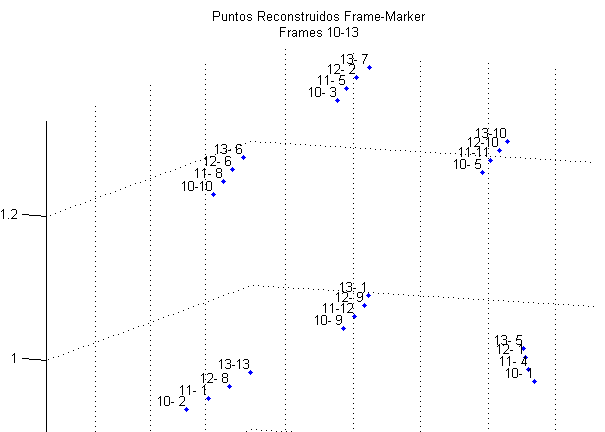
\includegraphics[scale=0.8]{img/Tracking/00_Salida_Reconstruccion.png}
\end{center}
\caption{Salida de Reconstrucción para 4 cuadros. La etiqueta para cada marcador es el cuadro y el índice en la reconstrucción}
\label{reconstr_00}
% Figura tomada de la reconstrucción 8_07_100_200
\end{figure}

\section{Estado del Arte}

El problema del seguimiento de marcadores espaciales a lo largo del tiempo es un tema de estudio habitual con distintos enfoques, entre ellos:

\begin{itemize}

\item Aplicación de restricciones al movimiento, teniendo información previa de los marcadores a estudiar, como se mueven, y como se relacionan entre ellos. 

\item Predictores Lineales o Estadísticos, teniendo información previa de una trayectoria para estimar el próximo elemento y confirmar o corregir la continuación de la secuencia.

\end{itemize}

Estos enfoques no son mutuamente excluyentes, pudiendo ser ambos complementarios para robustecer la generación de las trayectorias. Si se tiene acceso durante la adquisición de los datos, es posible relevar las distancias entre marcadores que se colocan en miembros que se mueven solidariamente  o dependen directamente uno del otro, por ejemplo al colocar marcadores en articulaciones de los brazos hay elementos sobre los huesos que siempre tendrán la misma distancia entre ellos (salvo una tolerancia, recordando que los marcadores no se encuentran en la articulación misma, sino sobre un lugar representativo sobre el cuerpo como se observa en el ajuste presentado en la Figura \ref{skeleton_fitting_herda} , como es planteado en el trabajo de Lorna Herda~\cite{herda}. ). Con estas distancias relevadas y definidas las relaciones entre marcadores, es posible definir el esqueleto como una serie de restricciones que se mantienen a lo largo del tiempo (distancias entre marcadores solidarios) o varían de forma continua (ángulo de huesos), donde la identificación es realizada inicialmente mediante un ajuste de los datos relevados en el mundo físico a los puntos obtenidos en la reconstrucción. 

\begin{figure}[hbt]
\begin{center}
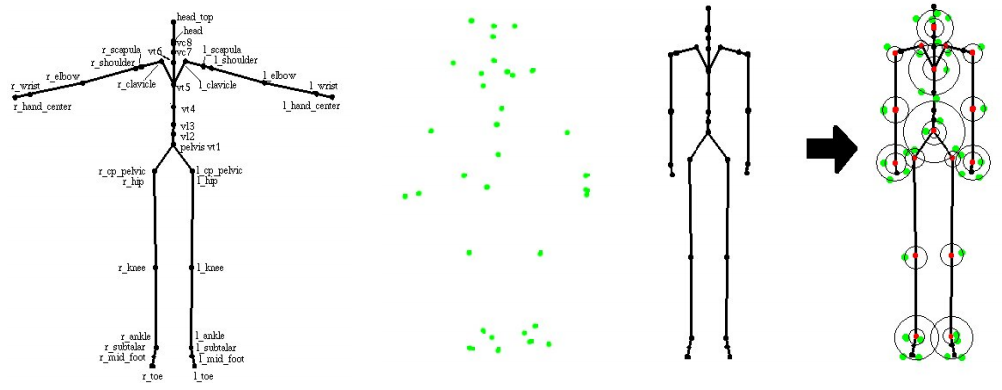
\includegraphics[scale=0.5]{img/Tracking/01_skeleton_fitting_Herda.png}
\end{center}
\caption{Inicialización de esqueleto, y ajuste a los marcadores encontrados. Cada marcador representa una articulación y se ajusta en una esfera de cercanía centrada en la articulación del esqueleto}
\label{skeleton_fitting_herda}
\end{figure}

Uno de los algoritmos mas simples~\cite{survey_tracking}, es continuar una secuencia buscando el marcador mas cercano al ultimo punto conocido imponiendo la restricción que el traslado es mínimo ("greedy matching"), pero es susceptible a errores para casos muy simples, como se observa en el ejemplo de la Figura \ref{greedy_matching} .

\begin{figure}[hbt]
\begin{center}
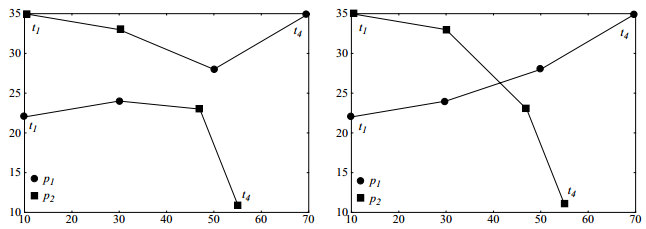
\includegraphics[scale=0.8]{img/Tracking/01_Greedy_Matching.png}
\end{center}
\caption{Dos marcadores moviéndose en cuatro cuadros, Izquierda corresponde al resultado de aplicar enlazado por elemento mas próximo~\cite{survey_tracking} , Derecha al elegir el camino con variación mas suave}
\label{greedy_matching}
\end{figure}

Para el caso de algoritmos de predicción, algunas soluciones implementadas para el tracking de marcadores en desarrollos similares como el DVIDEOW~\cite{figueroa2003flexible} son el filtro de Kalman~\cite{kalman}, y sus variantes los cuales requieren inicializar y ajustar parámetros internos. Estos fueron implementados en las primeras instancias del estudio del problema, pero se decidió implementar otro procedimiento que sepa corregir los errores del método mas simple, no requerir estudio de parámetros internos para el filtrado, e ingrese alguna restricción a las trayectorias enlazadas.
\\ 

El procedimiento elegido es el presentado por Lorna Herda~\cite{herda} , y consiste en aplicar el tracking de partículas esbozado por Malik,Dracos,Papantoniou~\cite{griegos} al seguimiento de marcadores. Este consiste en buscar el desplazamiento de un marcador desde el cuadro [f] al cuadro siguiente [f+1], sobre una ventana de cuatro cuadros.
\\ 

La hipótesis principal de este algoritmo, es que el muestreo del movimiento capturado es suficiente para que el desplazamiento entre cuadros sea mínimo en distancia, y la idea para predecir y buscar el desplazamiento entre [f] y [f+1], es utilizar la información que se tiene de la secuencia entre [f-1] y [f], y utilizar una segunda proyección entre [f+1] y [f+2] para confirmar el enlace encontrado en el caso que exista mas de una posibilidad (Figura~\ref{herda_00}).
\\ 

Para poder confirmar una trayectoria de 4 puntos, se debe cumplir que la misma presenta la menor variación de aceleración para la opción elegida entre todas las posibles, calculada como:

\begin{equation}
\begin{split}
\Delta{a}&= \left| \boldsymbol{\overrightarrow{a}}_{[f][f+1][f+2]}-\boldsymbol{\overrightarrow{a}}_{[f-1][f][f+1]} \right| \\
&= \left| \left(\boldsymbol{\overrightarrow{v}}_{[f+1][f+2]}-\boldsymbol{\overrightarrow{v}}_{[f][f+1]}\right).\Delta{t}-\left(\boldsymbol{\overrightarrow{v}}_{[f][f+1]}-\boldsymbol{\overrightarrow{v}}_{[f-1][f]}\right).\Delta{t} \right| \\
&= \left|\left( x_{[f+2]} - 3.x_{[f+1]} + 3.x_{[f]} - x_{[f-1]} \right).\Delta{t}^2\right|\\
\end{split}
\label{track_var_acc}
\end{equation}

donde $x_{[f+1]}$ a su vez, es aquel punto de [f+1] que mejor se aproxima al desplazamiento en cuadros anteriores, minimizando la Ecuación~\ref{track_acc} 

\begin{equation}
\begin{split}
\boldsymbol{\overrightarrow{v}}_{[f][f+1]}& = \boldsymbol{\overrightarrow{v}}_{[f-1][f]} \\
x_{[f+1]}-x_{[f]}& = x_{[f]}-x_{[f-1]} \\
\end{split}
\label{track_acc}
\end{equation}

\begin{figure}[hbt]
\begin{center}
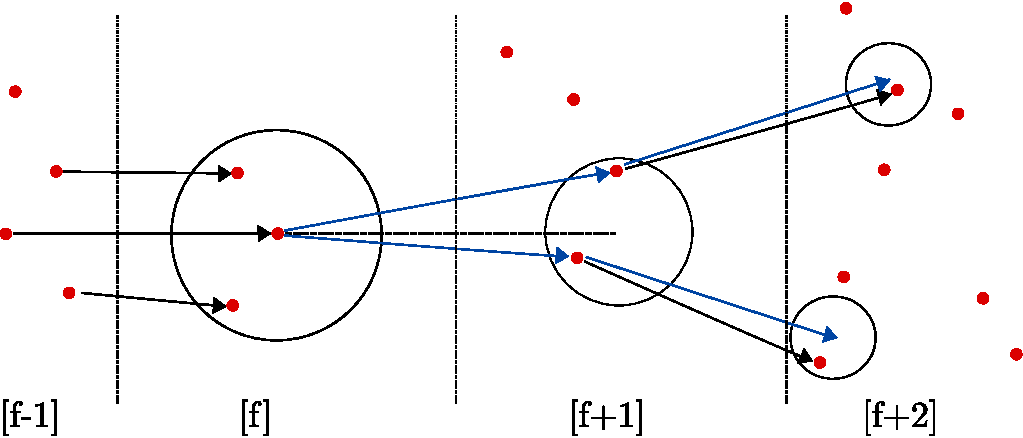
\includegraphics[scale=0.8]{img/Tracking/tracking-eps-converted-to.pdf}
\end{center}
\caption{Seguimiento en 4 cuadros, siendo [f] el cuadro actual que queremos seguir en [f+1]. La linea punteada es la traslación del movimiento previo, las lineas azules son las obtenidas buscando la mínima variación de aceleración para el punto elegido en [f+1]. De las dos posibles trayectorias, se elige aquella con menor variación de aceleración}
\label{herda_00}
\end{figure}

En su trabajo~\cite{herda}, Lorna Herda propone que realizar el seguimiento sobre la reconstrucción 3D presenta menos continuidad en las trayectorias , con respecto al seguimiento realizado sobre el conjunto de segmentación sumada a la proyección de los puntos reconstruidos 3D en cada vista 2D. Sin embargo, en nuestras pruebas, nos pareció mas coherente trabajar con el seguimiento en los puntos reconstruidos en 3D, ya que en caso de trayectorias que se cruzan en una vista 2D, son fácilmente separadas en 3D debido a la geometría.
\\ 

Adicionalmente, la reconstrucción fue implementada de forma distinta a la propuesta por Herda, si bien es posible obtener los puntos proyectados en cada vista, no cumplen el mismo rol. Sin implementar la re-proyección, en el tracking sobre una vista individual se pierden trayectorias cuando se pierden de vista como se observa en la Figura~\ref{tracking_2D_cam_07} .

\begin{figure}[hbt]
\begin{center}
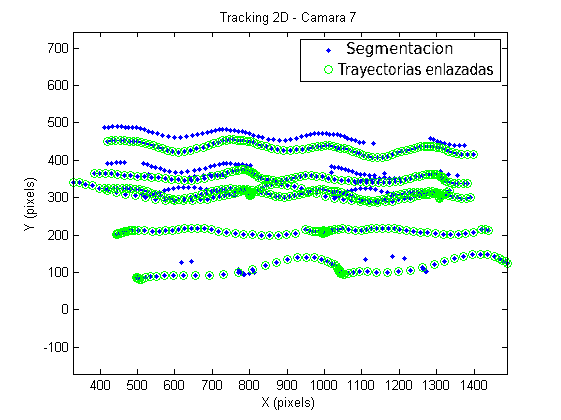
\includegraphics[scale=0.7]{img/Tracking/011_tracking_2D_camara_07.png}
\end{center}
\caption{Resultado de Aplicar el Seguimiento de marcadores a una vista 2D sin re-proyección de puntos reconstruidos. Verde, las trayectorias que se enlazaron completamente, Azul los puntos segmentados en la vista 2D de la cámara 07 de la captura sintética}
\label{tracking_2D_cam_07}
\end{figure}

Finalmente, asumiendo que los puntos obtenidos directamente de las animaciones ,proyectados en cada cámara, son el mejor caso de puntos 2D, no presentaban grandes ventajas de trabajar el enlace en cada una de estas vistas 2D, sobre trabajar en 3D posteriormente a la reconstrucción, y no volver hacia atrás ya que la geometría entre vistas cumplió su cometido. Esto ultimo no se cumple para el caso que se evalúen medidas adicionales para robustecer la salida del tracking (por ejemplo, validación por visibilidad, un punto observado en la segmentación de una vista es descartado en caso de no ser físicamente posible ver ese punto entre el cuerpo y la cámara).

\section{Implementación}

Para un cuadro [f] y un marcador $m_{i}^{[f]}$, se desea encontrar en el cuadro [f+1] el marcador $m_{j}^{[f+1]}$ que continúe la trayectoria que se tiene hasta el momento, cumpliendo las ecuaciones de continuidad~\ref{track_acc} y~\ref{track_var_acc}. El elemento que traslada la información de un cuadro al siguiente y desde el anterior, es la matriz de enlaces, donde cada linea es un enlace, y cada enlace tiene los siguientes elementos:
\begin{equation}
\begin{bmatrix}
  m_{h}^{[f-1]} ,\quad m_{i}^{[f]} ,\quad m_{j}^{[f+1]} ,\quad m_{k}^{[f+2]} ,\quad \left|\boldsymbol{\overrightarrow{a}}_{[f-1][f][f+1]}\right| ,\quad \left|\boldsymbol{\overrightarrow{v}}_{[f][f+1]}\right|
\end{bmatrix}
\end{equation}

Para el ejemplo presentado en la Figura~\ref{reconstr_00} , en cuadro $f=11$ el marcador $m=8$ presenta el siguiente enlace hacia $(f+1)=12$, donde el índice en [13] no aplica debido a que no fue necesario para establecer en enlace entre [11][12].

\begin{equation}
\begin{bmatrix}
  m_{3}^{[10]} ,\quad m_{8}^{[11]} ,\quad m_{3}^{[12]} ,\quad N/A ,\quad \left|\boldsymbol{\overrightarrow{a}}_{[10][11][12]}\right| ,\quad \left|\boldsymbol{\overrightarrow{v}}_{[1][12]}\right|
\end{bmatrix}
\end{equation}

Al final de cada iteración, la matriz de enlaces es consolidada para asignarle a cada nuevo marcador en [f+1] la etiqueta definida en el primer cuadro del enlazado, la cual puede ser inicializada como texto, si se le presenta la opción al usuario (en caso contrario, se utiliza el orden de los marcadores en el primer cuadro). Esta asignación será la que se utilice a lo largo de todo el seguimiento, por lo que todo marcador que no sea reconstruido en los primero cuadros, salvo de tomen medidas adicionales, no aparecerán en las trayectorias finales.

\subsection{Enlazado en régimen, inicial y final}

Dado un cuadro [f], se cargan todos los marcadores de los cuadros [f-1],[f],[f+1],[f+2], los cuales son puntos en coordenadas cartesianas $X,Y,Z$ (si el seguimiento desea hacerse para una vista 2D, se establece la tercer coordenada de todos los en valor predefinido unitario) en unidades correspondiente al plano donde se trabaja (píxeles para vistas 2D, metros para espacio 3D). Dentro de cada cuadro, los marcadores son identificados según su índice en la salida del algoritmo correspondiente, y los enlaces de cada marcador [f-1][f], son cargados a partir de la matriz de enlace del cuadro anterior (la segunda y tercer columna de la matriz de enlace de [f-1], presenta los mismos datos que la primer y segunda columna de la matriz de enlace en [f], salvo el orden en que es presentada que es asociado al cuadro en curso).

Para el $i$-esimo marcador en [f], se relevan los índices que componen el enlace [f-1][f] para obtener el traslado previo, y aplicarlo para obtener el centro de búsqueda para el marcador en [f], cumpliendo la Ecuación~\ref{track_acc} .

\begin{equation}
\begin{split}
\boldsymbol{\overrightarrow{v}}_{[f][f+1]}^{i} = \boldsymbol{\overrightarrow{v}}_{[f-1][f]}^{i} \Rightarrow C_{[f+1]}^{i} &= x_{[f]}^{i} + \boldsymbol{\overrightarrow{v}}_{[f-1][f]}^{i}.\Delta{t} \\
&= 2.x_{[f]}^{i} -x_{[f-1]}^{i} 
\end{split}
\label{centro_busqueda_f1}
\end{equation}

La norma de este traslado es utilizada para evaluar los puntos cercanos al centro de búsqueda, donde pueden surgir tres casos:

\begin{itemize}
\item Se encuentra un solo punto dentro del radio de búsqueda , se agrega el índice del punto encontrado en [f+1] a los que se utilizaron de [f-1] y [f], calculando la aceleración y velocidad resultante para establecer el enlace. En este caso, el cuarto elemento de la linea de la matriz de enlace, no fue necesario 
\item Se encuentra mas de un punto, por lo cual se tiene que usar algún criterio para elegir entre todas la posibilidades encontradas. Para cada punto encontrado dentro del radio de búsqueda, se calcula un segundo centro de búsqueda para [f+2], esta vez minimizando la Ecuación~\ref{track_var_acc} :
\begin{equation}
\begin{split}
\boldsymbol{\overrightarrow{a}}_{[f][f+1][f+2]}=\boldsymbol{\overrightarrow{a}}_{[f-1][f][f+1]} \Rightarrow C_{[f+2]}^{i} &= x_{[f+1]}^{i} + \boldsymbol{\overrightarrow{v}}_{[f][f+1]}^{i}.\Delta{t} + \boldsymbol{\overrightarrow{a}}_{[f-1][f][f+1]}^{i}.\Delta{t}^2\\
&= 3.x_{[f+1]}^{i} - 3.x_{[f]}^{i} + x_{[f-1]}^{i}\end{split}
\label{centro_busqueda_f2}
\end{equation}
Siendo el radio de búsqueda en [f+2], la distancia [f][f+1]. Con los puntos encontrados en cada búsqueda de todas las posibilidades, se evalúa la variación de aceleración para los puntos [f-1][f][f+1][f+2], y elige la menor de todas, estableciendo el enlace de 4 puntos. Finalmente, se calcula la aceleración y velocidad del enlace [f-1][f][f+2], y se guardan los índices que permitieron la decisión, esta vez con cuatro elementos para indicar que se procedió con la segunda búsqueda.
\item No se encuentra ningún punto, tanto para la búsqueda en [f+1] como en [f+2]. En este caso, se presentan múltiples alternativas, en distintas etapas. La mas inmediata durante el enlazado cuadro a cuadro, es aumentar el radio de búsqueda (por ejemplo puede suceder con un punto acelerando y fuera del radio de búsqueda). Este aumento puede ser limitado, o indefinido hasta encontrar un punto aunque en una distancia mucho mayor a la esperada, por lo que deben ser validados posteriormente. Si el enlace pasa la validación dentro del cuadro, puede no pasar una validación posterior de trayectoria lo que se verá mas adelante
\end{itemize}

El enlazado final es similar a los presentado para régimen, pero en caso de múltiples marcadores candidatos en el cuadro final [f+1], no se puede extender el movimiento, por lo que se elige mediante menor aceleración en los últimos tres cuadros con una sola búsqueda desde [f] a [f+1], pero otra alternativa igualmente valida hubiera sido buscar sobre los últimos cuatro cuadros. Se eligió la primer opción debido a  ser un caso simplificado del enlazado en régimen ya implementada. 
\\ 

Sin embargo, el enlazado inicial presenta una situación diferente, no se tiene información previa, y deben establecerse las bases para el inicio del enlazado. Para ello se cargan todos los marcadores en los primeros 3 cuadros, se calculan todas las posibles combinaciones de trayectorias entre elementos. En caso de existir combinaciones forzadas invalidas, las mismas presentan una aceleración resultante notoriamente mayor a la de enlaces, pero si corresponden a algún punto erróneo este se perderá naturalmente durante el enlazado,
\\ 

Una vez enlazado el ultimo cuadro de las secuencia, se procede a limpiar aquellas trayectorias que perdieron marcadores en el camino estableciendo un umbral de perdida aceptables sobre el largo de las secuencias obtenidas. Adicionalmente, se descartan todos los puntos reconstruidos que no fueron asignados a ninguna trayectoria 


\subsection{Validación e Inventario de trayectorias}

Antes de consolidar la matriz de enlaces y proceder a que los marcadores en [f+1] hereden las etiquetas de las trayectorias a las que pertenecen, los enlaces deben ser validados en múltiples instancias:

\begin{itemize}
\item \textbf{Validación dentro del cuadro}: verificar que los índices de la matriz de enlaces en [f+1] son únicos, asociados a una sola trayectoria. Si dos o mas trayectorias se enlazaron a un mismo punto en [f+1], se comparará la aceleración con la que fueron enlazadas, validando aquella con menor aceleración, y descartando las otras. En este punto , existe la posibilidad de haber agregado todas las trayectorias involucradas en la decisión en vez de una sola trayectoria por marcador en [f+1], que mejor cumplía las condiciones para ese marcador. De haber elegido esta opción, el descartar una trayectoria que podría haber sido elegida por menor variación , daría paso a la siguiente mejor. Este caso sucedía mas en los casos que se aplico el seguimiento para trayectorias 2D, no tanto en 3D, por lo cual se terminó procediendo con solo una trayectoria por marcador, la cual en caso de ser invalida debe ser evaluada en la etapa de inventario de trayectorias  
\item \textbf{Validación en trayectoria}: pueden existir puntos que fueron reconstruidos con leves errores que deben detectarse, corregirse y estimar un reemplazo. Estos puntos son detectados como enlazados correctamente, pero con posición, velocidad, o aceleración que presenta una discontinuidad notoria, como puede observarse en el ejemplo de la Figura~\ref{discontinuidad_tracking}.

\begin{figure}[H]
 \centering
  \subfloat[Trayectoria]{
   \label{track_m13}
    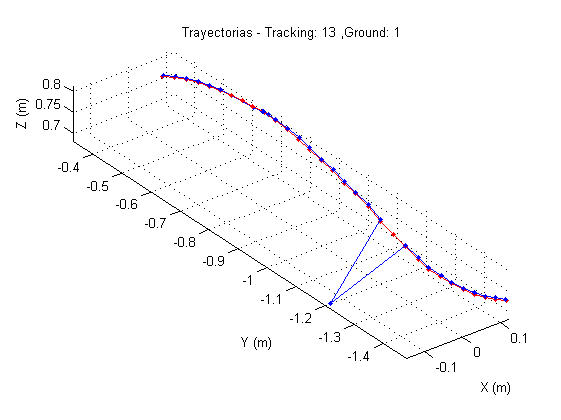
\includegraphics[width=0.5\textwidth]{img/Tracking/025_Salida_Tracking_Marker_13_8_07_100_200.png}}
  \subfloat[Velocidad,Aceleración,Variación Ac.]{
   \label{vel_acc_vacc_m13}
    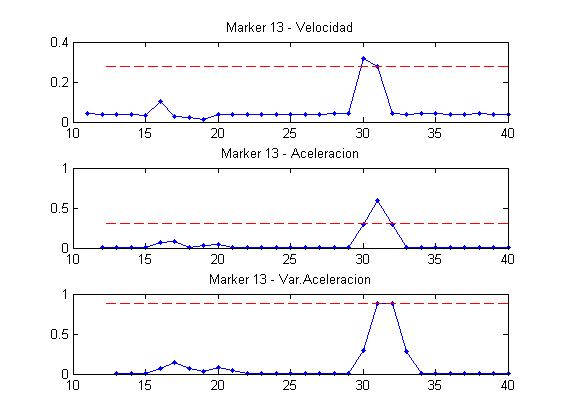
\includegraphics[width=0.5\textwidth]{img/Tracking/020_Salida_Tracking_Marker_13_8_07_100_200.png}}
 \caption{Ejemplo de discontinuidad en un marcador, por punto mal reconstruido. La Figura~\ref{track_m13} presenta en azul la trayectoria reconstruida, en rojo el ground truth}
 \label{discontinuidad_tracking}
\end{figure}

Se establece un umbral a partir del estudio de la distribución de la aceleración de cada marcador (Figura~\ref{distribucion_aceleracion} ) para encontrar la aceleración que presenta un salto abrupto, y detectar los cuadros donde se supera dicho umbral para corregir el marcador. El procedimiento para estimar los marcadores en estos casos, es el mismo que se verá al momento de inventario de trayectorias. 
\\ 

Como opción general, se implementó una alternativa que en vez de calcular un umbral para cada trayectoria, establece un umbral global, el cual es útil para detectar aceleraciones notoriamente altas sin tener que estudiar cada trayectoria. Esta opción se logra mediante una ejecución en dos instancias del seguimiento, una primera instancia sin limites globales de aceleración en en enlazado, y una segunda con un limite establecido a un porcentaje de la distribución de la aceleración, asumiendo un nivel a priori para perdidas (en nuestras pruebas, se estableció que filtrar al nivel que cumplan el 99\% de las aceleraciones de todos los marcadores enlazados arroja buenos resultados). Si durante la segunda instancia, un enlace global supera este umbral, se descarta y se procede con la recuperación de trayectoria.

\begin{figure}[H]
 \centering
  \subfloat[Función de distribución de la Aceleración]{
	\label{distribucion_aceleracion}
	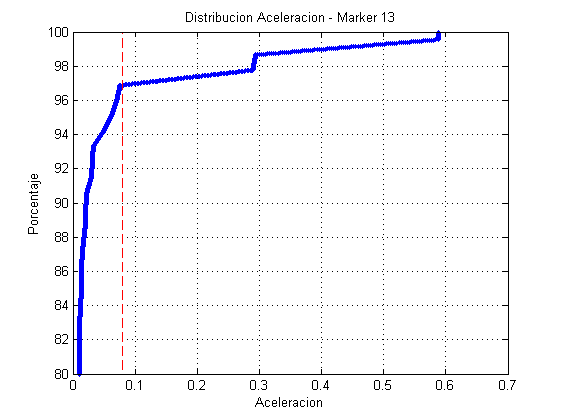
\includegraphics[width=0.5\textwidth]{img/Tracking/03_Distribucion_Aceleracion_Marker_13_8_07_100_200.png}}
  \subfloat[]{
   \label{track_m13_fix}
    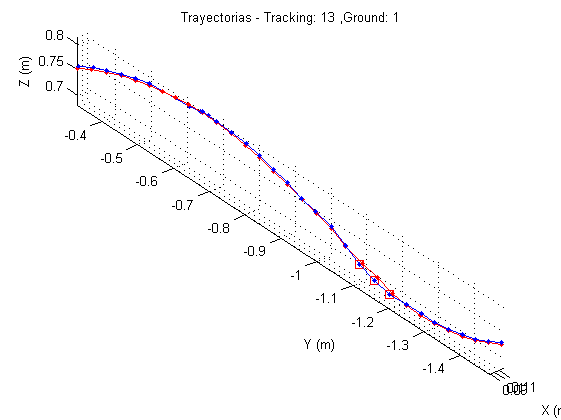
\includegraphics[width=0.5\textwidth]{img/Tracking/026_Salida_Tracking_Marker_13_8_07_100_200.png}}
 \caption{Ejemplo Resultado de Umbral y Corrección En Trayectoria}
% Figura tomada de la reconstrucción 8_07_100_200
\label{distro_acc_track_m13_fix}
\end{figure}
\item \textbf{Inventario de Trayectorias}: Durante el enlazado en un cuadro, se tienen marcadores en [f] que no lograron enlazarse en [f+1], pero cuya trayectoria podría estar enlazada hasta este cuadro.
Estos puntos deben ser identificados, mediante la comparación de la segunda columna de la matriz de enlaces [f][f+1] (actual) y la tercer columna de la matriz de enlaces [f-1][f] (anterior), ya que ambas tienen información de los marcadores en el mismo cuadro, pero enlazan hacia atrás y adelante.
Los elementos que se encuentren en la matriz [f-1][f] , pero no hayan sido enlazados en [f][f+1], son agregados a una lista que  contiene hasta que momento el cuadro mantenía el enlace (ultima vez que se tuvo información de la trayectoria a la cual pertenece), y que índice de marcador tenia en ese momento (pasar de índice en un cuadro, a trayectoria a la cual pertenece es trivial consultando las etiquetas de marcador que se van heredando de cuadro a cuadro).
Una vez actualizada la lista de las trayectorias perdidas en [f][f+1], se deben tratar de enlazar los puntos de [f+1] que no entraron en el enlazado regular, con las trayectorias perdidas hasta [f-1]. Todos los puntos que sobraron en el enlazado regular, son evaluados contra la lista de trayectorias perdidas, y se revisan dos condiciones:

\begin{enumerate}
  \item \textbf{Distancia con respecto a una estimación lineal}, prolongando el movimiento tomando el ultimo punto como inicio, y los últimos cuadros de la trayectoria conocida como desplazamiento. El desplazamiento es repetido tantas veces como tiempo perdido tiene el marcador: si una trayectoria estaba definida hasta [f-1] y se buscan enlaces con elementos de [f+1], el desplazamiento es repetido dos veces, como puede observarse en el ejemplo de la Figura~\ref{track_m8_recover}. 
 
\begin{figure}[H]
 \centering
  \subfloat[Salida de Código durante perdida y recuperación de trayectoria]{
	\label{track_m8_recover_code}
	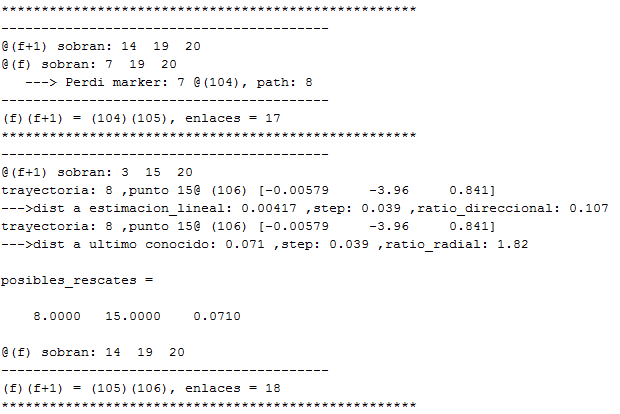
\includegraphics[scale=0.7]{img/Tracking/035_Salida_Codigo_Recuperacion.png}}\hspace{3 mm}
	
  \subfloat[Trayectoria]{
   \label{track_m8_recover}
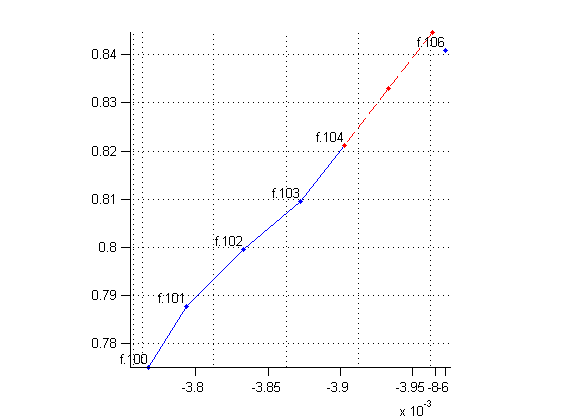
\includegraphics[scale=0.7]{img/Tracking/030_Inventario_trayectoria_direccional.png}}
\caption{Trayectoria perdida en cuadro 104, con posible candidato de recuperación en cuadro 106 por cercanía con la estimación por desplazamiento}
% Figura tomada de la reconstrucción 8_07_100_200
\label{inventario_trayectoria_direccional}
\end{figure} 
  
  \item \textbf{Distancia radial con respecto al ultimo punto conocido}. En algunos casos, la perdida del enlazado puede suceder cuando la trayectoria está en reposo (por ejemplo, un pie apoyado antes de volver a despegarse del suelo), o en transición (en el medio de una curva), por lo cual la estimación lineal anterior es invalida. Para ello, es útil relevar la distancia entre el ultimo punto conocido de una trayectoria trunca, y los puntos que no se enlazaron en [f+1]. Esta distancia, en caso de una posible recuperación, deberá ser proporcional al ultimo traslado conocido, por la diferencia temporal de cuadros entre el ultimo punto, y el posible candidato.
 
El procedimiento de validación indica que marcadores son inválidos, tanto usando el umbral global, como el individual, pero esta validación puede truncar una trayectoria durante el enlazado que luego debe ser estimada en caso de recuperación, o debe ser filtrado para el caso de post-procesamiento. Se debe establecer un procedimiento para tratar de recuperar estos marcadores, tratando de cumplir con las restricciones impuestas.
 
  
\end{enumerate} 

\end{itemize}

\subsection{Estimación de Marcadores Perdidos Durante Enlazado}

Si se encuentra algún punto que cumpla alguna de las condiciones de recuperación de trayectorias, es considerado para continuar la trayectoria, y deben estimarse los puntos intermedios para completar la trayectoria.
\\ 

Esta estimación es realizada mediante mínimos cuadrados, donde las condiciones iniciales dependen de cuantos puntos de la trayectoria se tenían hasta el momento, la condición final es el punto encontrado en [f+1], las incógnitas son los puntos intermedios que se quieren encontrar, y las múltiples ecuaciones a cumplir son las planteadas en (\ref{track_var_acc}) y (\ref{track_acc}).
\\ 

Sea $X_{[f+1]}$ un punto candidato por las condiciones anteriores, y el ultimo punto conocido en [f-1] de un trayectoria que pretende continuar, verifica [f-1]$\geq$3, entonces las ecuaciones que el punto a estimar $\boldsymbol{\tilde{X}_{[f]}}$ deberá cumplir, (observar que las ecuaciones de variación de aceleración son combinación lineal de las ecuaciones de aceleración)

\begin{equation}
\left\{
\begin{matrix}
X_{[f-3]} &-3.X_{[f-2]} &+3.X_{[f-1]} &-\boldsymbol{\tilde{X}_{[f]}} & &=0 \\
 &X_{[f-2]} &-3.X_{[f-1]} &+3.\boldsymbol{\boldsymbol{\tilde{X}_{[f]}}} &-X_{[f+1]} &=0 \\
 &X_{[f-2]} &-2.X_{[f-1]} &+\boldsymbol{\boldsymbol{\tilde{X}_{[f]}}} & &=0 \\
 & &X_{[f-1]} &-2.\boldsymbol{\boldsymbol{\tilde{X}_{[f]}}} &+X_{[f+1]} &=0 \\
\end{matrix}
\right.
\label{ecuaciones_estimacion_01}
\end{equation}

Escribiendo de forma matricial, separando los datos en incógnitas y condiciones,

\begin{equation}
\hspace{-3.5cm}
\begin{split}
&\begin{pmatrix}
1 &-3 &3 &-1&0\\
0 &1 &-3 &3 &-1\\
0 &1 &-2 &1 &0\\
0 &0 &1 &-2 &1\\
\end{pmatrix}
\begin{pmatrix}
X_{[f-3]}\\
X_{[f-2]}\\
X_{[f-1]}\\
\boldsymbol{\tilde{X}_{[f]}}\\
X_{[f+1]}\\
\end{pmatrix} = 
\begin{pmatrix}
1 &-3 &3\\
0 &1 &-3\\
0 &1 &-2\\
0 &0 &1\\
\end{pmatrix}
\begin{pmatrix}
X_{[f-3]}\\
X_{[f-2]}\\
X_{[f-1]}\\
\end{pmatrix}+
\begin{pmatrix}
-1\\
3\\
1\\
-2\\
\end{pmatrix}
\boldsymbol{\tilde{X}_{[f]}}+
\begin{pmatrix}
0\\
-1\\
0\\
1\\
\end{pmatrix}
X_{[f+1]} = 
\begin{pmatrix}
0\\
0\\
0\\
0\\
\end{pmatrix} \\
&\Rightarrow
\underbrace{
\begin{pmatrix}
-1\\
3\\
1\\
-2\\
\end{pmatrix}
}_{A_{[f]}}\boldsymbol{\tilde{X}_{[f]}} = \underbrace{- \begin{pmatrix}
1 &-3 &3\\
0 &1 &-3\\
0 &1 &-2\\
0 &0 &1\\
\end{pmatrix}
\begin{pmatrix}
X_{[f-3]}\\
X_{[f-2]}\\
X_{[f-1]}\\
\end{pmatrix} - \begin{pmatrix}
0\\
-1\\
0\\
1\\
\end{pmatrix}
X_{[f+1]}}_{B_{[f]}} \\
&\Rightarrow \boldsymbol{\tilde{X}_{[f]}} = \left( A_{[f]}^{t}.A_{[f]}\right)^{-1}.A_{[f]}^{t}.B_{[f]}
\end{split}
\label{matrices_estimacion_01}
\end{equation}

El procedimiento presentado para aproximación de puntos es análogo para el caso de tener $n$ cuadros a estimar entre el ultimo momento $f_{i}$ de una trayectoria, y su posible continuación en $f_{j}$, con $n+1=f_{j}-f_{i}$. Si $f_{i} \geq 3$ , se plantearán $n+1$ ecuaciones para variación de aceleración, y $n+1$ ecuaciones para variación de velocidad (aceleración), las cuales se resuelven de la misma forma. 

\begin{equation}
\hspace{-2cm}
\left\{
\begin{matrix}
X_{[f_{i}-2]} &-3.X_{[f_{i}-1]} &+3.X_{[f_{i}]} &-\boldsymbol{\tilde{X}_{[f_{i}+1]}} & & & &=0 \\
& X_{[f_{i}-1]} &-3.X_{[f_{i}]} &+3.\boldsymbol{\tilde{X}_{[f_{i}+1]}} &-\boldsymbol{\tilde{X}_{[f_{i}+2]}} & & &=0 \\
& & X_{[f_{i}]} &-3.\boldsymbol{\tilde{X}_{[f_{i}+1]}} &+3.\boldsymbol{\tilde{X}_{[f_{i}+2]}} &-\boldsymbol{\tilde{X}_{[f_{i}+3]}}& &=0 \\
& & & \ddots & \ddots & \ddots & \ddots & \\
& & & \boldsymbol{\tilde{X}_{[f_{j}-3]}} &-3.\boldsymbol{\tilde{X}_{[f_{i}-j]}} &+3.\boldsymbol{\tilde{X}_{[f_{j}-1]}} &-X_{[f_{j}]} &=0 \\
\end{matrix}
\right.
\label{ecuaciones_estimacion_n}
\end{equation}

En caso que la información previa a la perdida es menor, con $f_{i} \geq 2$, se plantea una ecuación menos, aquella que plantea la variación de aceleración de aceleración con el primer elemento incógnita que es la única que precisaría tres elementos previos, las otras ecuaciones no tienen problemas para plantearse.

Esta metodología de estimación de puntos intermedios es retomada para la validación en trayectoria, donde las incógnitas pasan a ser lo puntos que deben ser regularizados debido a presentar aceleración excesiva y discontinua para el marcador ( como fue establecido al principio de esta sección).




\section{Resultados y Análisis}

El objetivo del bloque de seguimiento es identificar los puntos reconstruidos, presentarlos como trayectorias, y corregirlos si es necesario. Por esta razón, es esperable que para una misma secuencia, los resultados sean similares a la reconstrucción, siendo las únicas leves diferencias las correcciones realizadas sobre trayectorias particulares, y la posibilidad de medir el error por marcador individual ya que a esta altura del algoritmo ya están identificados las distintas trayectorias. Los siguientes resultados fueron probados sobre una captura sintética de 113 cuadros, 14 marcadores, a lo largo de 17 cámaras.

\begin{figure}[hbt]
\begin{center}
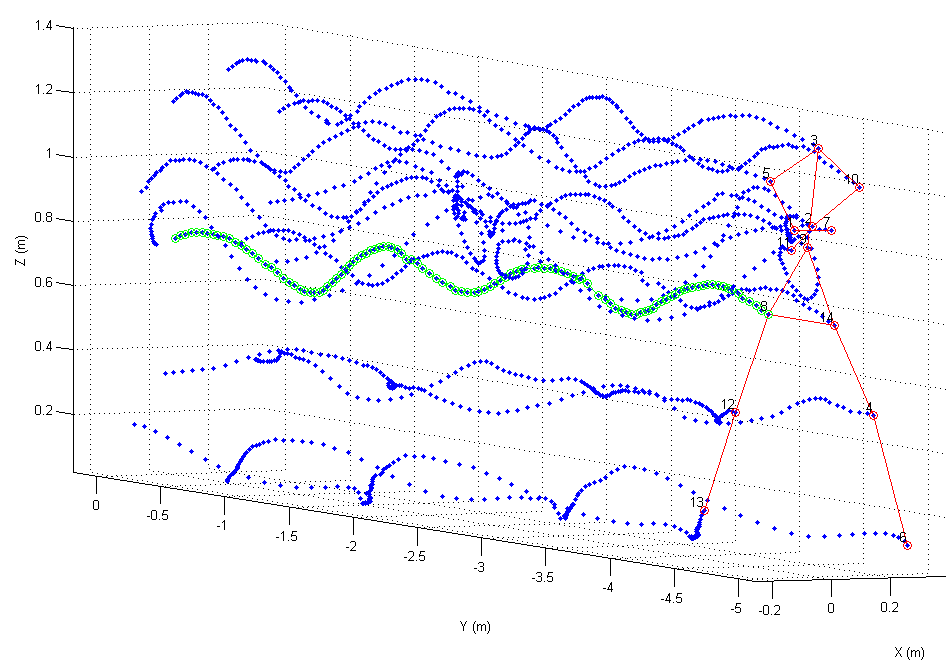
\includegraphics[width=\linewidth]{img/Tracking/040_Salida_Tracking_Esqueleto_Trayectoria.png}
\end{center}
\caption{Tracking sobre captura sintética, 113 cuadros, 17 cámaras, 14 marcadores}
\label{Tracking_Esqueleto_Trayectoria}
\end{figure}

El filtrado y validación por trayectorias, permite reducir el error máximo y mejorar el promedio de trayectorias especificas (marcador 8 en figura), pero al aplicar global mente puede perjudicar a aquellas trayectorias que tengan naturalmente discontinuidades en aceleración debido a variaciones abruptas de movimiento (Tabla \ref{tablaerrortrack}). Para todos los marcadores, el error promedio se encuentra por debajo de 0.5 cm para la reconstrucción sobre vídeos sintéticos de la secuencia CMU-8-07-100-200 con 17 cámaras, y con el filtrado por aceleración individual de marcadores. En otras capturas, los comportamientos son similares con promedios inferiores a 0.5 cm, y errores máximos por debajo de 3 cm, para el caso de reconstrucción con 17 cámaras.Mas adelante se estudiará el impacto de cambiar los conjunto de cámaras en marcadores   

\begin{table}[h]
\resizebox{15cm}{!}{
\begin{tabular}{|c|c|c|c|c|c|c|}
\hline
\begin{tabular}[c]{@{}c@{}}Marker\\ Track\end{tabular} & \begin{tabular}[c]{@{}c@{}}Marker\\ Ground\end{tabular} & \begin{tabular}[c]{@{}c@{}}Name\\ Ground\end{tabular}       & \begin{tabular}[c]{@{}c@{}}Error\\ Promedio(cm)\end{tabular} & \begin{tabular}[c]{@{}c@{}}Percentil\\ 99\%(cm)\end{tabular} & \begin{tabular}[c]{@{}c@{}}Error Promedio\\ (filtrado)(cm)\end{tabular} & \begin{tabular}[c]{@{}c@{}}Percentil 99\%\\ (filtrado)(cm)\end{tabular} \\ \hline
12       & 1         & LeftUpLeg          & 0,3671                                                       & 0,5158                                                       & 0,4042                                                                  & 2,0371                                                                  \\ \hline
3        & 2         & LeftLeg            & 0,367                                                        & 0,5411                                                       & 0,5456                                                                  & 2,7576                                                                  \\ \hline
2        & 3         & LeftFoot           & 0,372                                                        & 0,558                                                        & 0,377                                                                   & 0,7558                                                                  \\ \hline
6        & 4         & RightUpLeg         & 0,3714                                                       & 0,5879                                                       & 0,4033                                                                  & 1,6849                                                                  \\ \hline
4        & 5         & RightLeg           & 0,378                                                        & 0,586                                                        & 0,446                                                                   & 2,1396                                                                  \\ \hline
14       & 6         & RightFoot          & 0,4212                                                       & 1,8483                                                       & 0,4447                                                                  & 1,8483                                                                  \\ \hline
9        & 7         & Spine              & 0,404                                                        & 0,6043                                                       & 0,4103                                                                  & 0,7652                                                                  \\ \hline
7        & 8         & Head               & 0,3867                                                       & 0,9063                                                       & 0,3923                                                                  & 1,2422                                                                  \\ \hline
8        & 9         & LeftArm            & 0,3666                                                       & 0,7997                                                       & 0,3617                                                                  & 0,594                                                                   \\ \hline
13       & 10        & LeftForeArm        & 0,3873                                                       & 0,9056                                                       & 0,3961                                                                  & 1,1897                                                                  \\ \hline
10       & 11        & LeftHand           & 0,4007                                                       & 1,1722                                                       & 0,4128                                                                  & 1,4842                                                                  \\ \hline
1        & 12        & RightArm           & 0,4025                                                       & 1,4771                                                       & 0,3866                                                                  & 0,944                                                                   \\ \hline
11       & 13        & RightForeArm       & 0,3844                                                       & 0,781                                                        & 0,3945                                                                  & 0,8591                                                                  \\ \hline
5        & 14        & RightHand          & 0,3816                                                       & 0,7728                                                       & 0,411                                                                   & 1,1087                                                                  \\ \hline
         &           & \textbf{Secuencia} & \textbf{0,35686}                                             & \textbf{0,81266}                                             & \textbf{0,38305}                                                        & \textbf{1,6747}                                                         \\ \hline
\end{tabular}
}
\caption{Medida de error de tracking en captura de la base de datos sintética.}
\label{tablaerrortrack}
\end{table}

\begin{figure}[H]
 \centering
  \subfloat[Trayectoria sin Corregir Por Aceleración]{
	\label{Salida_Tracking_Original}
	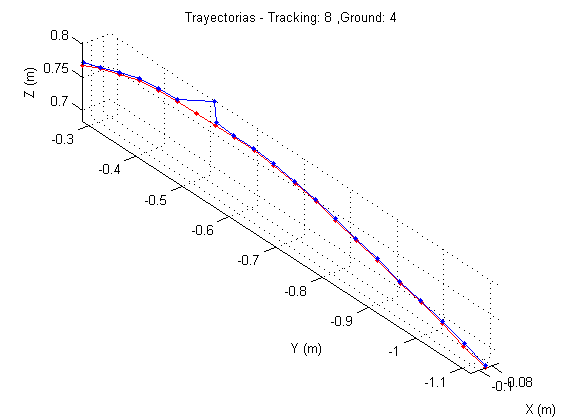
\includegraphics[scale=0.5]{img/Tracking/036_Salida_Tracking_Original.png}}
  \subfloat[Trayectoria Corregida Por Aceleración]{
   \label{Salida_Tracking_Filtrado}
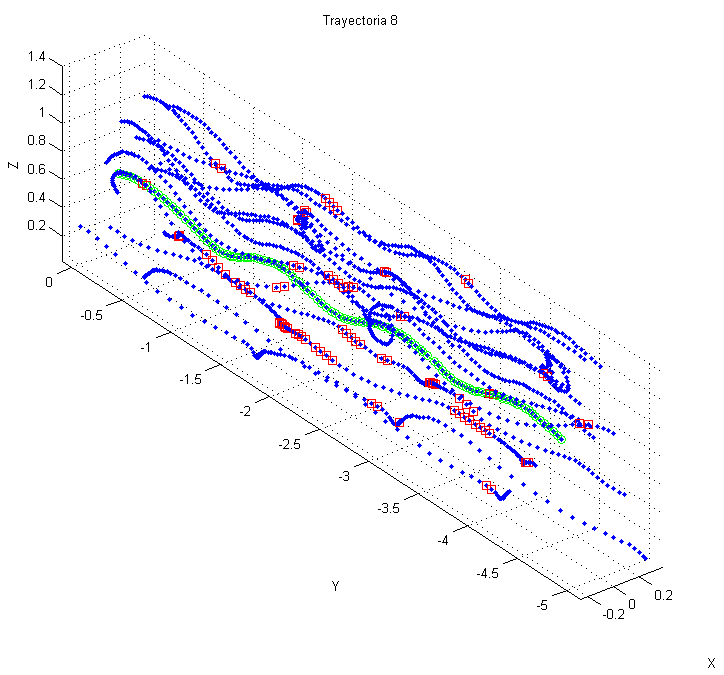
\includegraphics[scale=0.5]{img/Tracking/037_Salida_Tracking_Filtrado.png}}
\hspace{3 mm}
  \subfloat[Error de Marcador, sin Corregir]{
	\label{Salida_Tracking_Original2}
	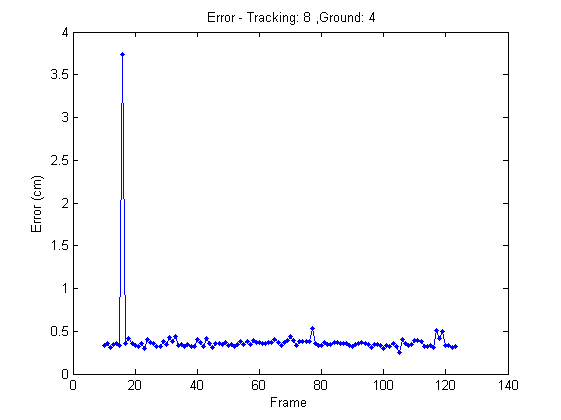
\includegraphics[scale=0.5]{img/Tracking/038_Salida_Tracking_Error_Marker_8_original.png}}
  \subfloat[Error de Marcador, Corregido]{
   \label{Salida_Tracking_Filtrado2}
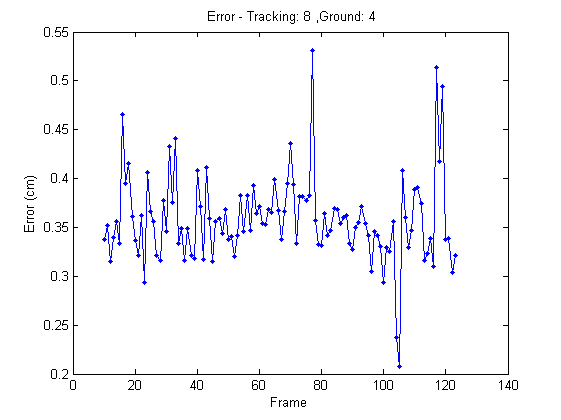
\includegraphics[scale=0.5]{img/Tracking/039_Salida_Tracking_Error_Marker_8_filtrado.png}}
\caption{Corrección por variación de aceleración, medidas de error antes y después de corregir}
% Figura tomada de la reconstrucción 8_07_100_200
\label{Tracking_Original_Filtrado_Errores}
\end{figure}


Al tener las etiquetas constantes para las trayectorias, es posible visualizar la relación entre marcadores, quedando pendientes medidas adicionales para robustecer el sistema, como imponer restricciones al movimiento entre marcadores en un mismo miembro, por imponer no solo continuidad en aceleración de marcadores sino ángulos de articulaciones y huesos. Esta continuidad debe tener cierta tolerancia debido a que los marcadores son representativos de articulaciones, y no se mueven completamente solidarios por lo que existen leves variaciones en las distancias entre marcadores, como se observa en la Figura \ref{distancia_angulo_marcadores_piernas}, correspondiente a los marcadores asociados a la pierna en la captura 8\_03\_100\_100. En este caso se observa la continuidad y periodicidad de el ángulo entre marcadores así como la constancia de la distancia, salvo momentos ocasionales, asociados a momentos específicos de la captura (cuando el pie rompe el reposo por ejemplo, antes de dar otro paso) ,sin ser mayor a los pocos centímetros en momentos puntuales y recuperables en régimen.

\begin{figure}[H]
 \centering
  \subfloat[Trayectorias de marcadores de pierna]{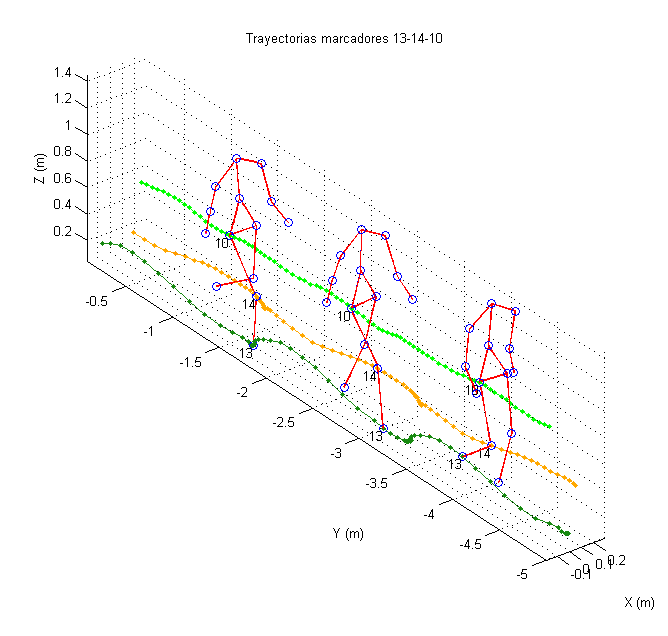
\includegraphics[scale=0.45]{img/Tracking/050_Salida_Tracking_13_14_10.png} %\label{trayectorias_marcadores_piernas}
   }	
  \subfloat[Distancia y Angulo entre marcadores de la pierna]{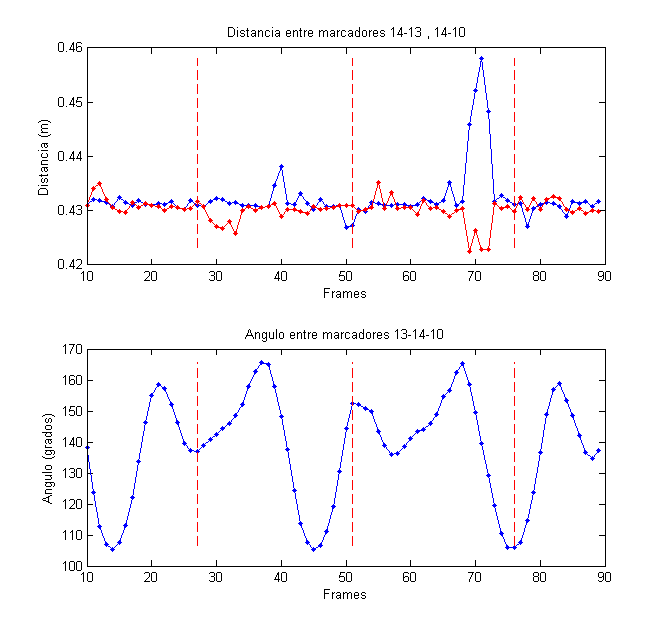
\includegraphics[scale=0.45]{img/Tracking/051_Salida_Angulo_Distancia_13_14_10.png}\label{distancia_angulo_marcadores_piernas}}
\caption{Ejemplos de Posibles restricciones en ángulo y distancia, para el caso de la pierna en marcha}
\label{restricciones_tracking}
\end{figure}
